\documentclass[a4paper,12pt]{article}

\usepackage{latexsym}
\usepackage[utf8]{inputenc}
\usepackage{graphicx}
\usepackage{amsmath}

\author{Krzysztof~Palka and Dominik~Odrowski}
\date{March 21, 2013}

\title{\textsc{Exercise} 532 \\ Electron diffraction on polycrystalline graphite lattice.} 

\addtolength{\textwidth}{2.5cm}
\addtolength{\hoffset}{-1.25cm}

\begin{document}

\maketitle

\begin{abstract}
This report presents examination of de Broglie's postulate concerning material particles and calculating of inter-planar spacing in graphite material. 
\end{abstract}

\section{Introduction}
The aim of this exercise was to determine interplanar spacing of graphite using Broglie's postulate about consideration beam of electrons as wave and, as source of data, electron diffraction vacuum tube. 

\section{Theory and measurement}
In 1924, physicist Louis de Broglie proposed extension of Einstein's suggestion that a quantum of light has linear momentum in the way that not only photons, but also electrons obey this phenomena \cite{HRW}.
According to this, electron's wavelength can be calculated from formula
\begin{equation}
    \lambda = \frac{h}{p} \label{eq:bwl}
\end{equation}
where $h$ is the Planck's constant and $\lambda$ is called de Broglie wavelength of the moving particle.

Considering beam of electrons as wave and using graphite as diffraction grading - accelerated by electron gun electrons are diffracted from a polycrystalline layer of graphite and shown on screen in form of luminous rings (Fig. \ref{fig:tube}), we can calculate, from the diameter of the rings and accelerating voltage interplanar spacing of the structure.

\begin{figure}[h]
\begin{center}
    \includegraphics[width=0.7\textwidth]{tube}
    \caption{Electron diffraction vacuum tube \cite{E21}. It consists of: graphite lattice (P); electron gun: cathode (K), Wehnelt cylinder (H), electronic lens system (G), focusing voltage regulator (U$_{1}$), stopping voltage regulator (U$_{2}$), anode (A); screen (E) and high voltage power supply (S).}
    \label{fig:tube}
\end{center}
\end{figure}

The momentum $p$ of particles can by calculated form velocity $v$
\begin{equation}
    E = \frac{mv^2}{2} = \frac{p^2}{2m} \label{eq:E1}
\end{equation}
where $m$ is rest mass of electron. Energy can by calculated also from acceleration voltage $U_A$
\begin{equation}
    E = eU_A \label{eq:E2}
\end{equation}
where $e$ is the electron charge. By combining equations \ref{eq:bwl}, \ref{eq:E1} and \ref{eq:E2} we can obtain following dependency.
\begin{equation}
    \lambda = \frac{h}{\sqrt{2mU_A}}  \label{eq:bwl2}
\end{equation}
Bragg equation (\ref{eq:bragg}) describes the reflection of the electron beam on the structural lattice of crystal
\begin{equation}
    2d\sin\theta = n\lambda  \label{eq:bragg}
\end{equation}
where $d$ is the spacing between layers of carbon's atoms and $\theta$ is the angle between incident beam and lattice planes (Bragg angle).
According to figure \ref{fig:tube}
\begin{equation}
    \sin 2\alpha = \frac{r}{R} \label{eq:ang1}
\end{equation}
where $r$ is the radius of the interference ring and $R$ is the radius of the glass bulb.
Assuming that for small angles of $\theta$: $\sin \alpha = \sin 2 \theta \approx 2 \sin \theta$ we can obtain
\begin{equation}
    r = \frac{2R}{d} n \lambda
\end{equation}

\section{Results}
From equation \ref{eq:bwl2} we can calculate wavelength, assuming that $h = 6.625 \cdot 10^{-34}$ Js and $m = 9.109 \cdot 10 ^ {-31}$ kg. And from equation \ref{eq:ang1} radii of the ring, assuming that the radius of the glass bulb, $R = 65 \cdot 10^{-3}$ m.
\begin{table}[h]
    \begin{center}
        \caption{Measured angles and calculated radii and wavelengths for setted voltages.}
        \label{tab:resoults}
        \begin{tabular}{|c|c|c|c|c|c|}
            \hline
            $2\alpha_1 [^\circ]$ & r$_1$ [$10^{-3}$m] & $2\alpha_2 [^\circ]$ & r$_2$ [$10^{-3}$m] & U$_A$ [kV] & $\lambda$ [$10^{-21}$m] \\
            first ring & first ring & second ring & second ring & anode & wavelength \\ 
            angle & radius & angle & radius & voltage & \\
            \hline 
            28 & 30.516 & 46 & 46.757 & 2.5 & 9.817 \\
            \hline
            36 & 38.206 & 44 & 45.153 & 3.0 & 8.961 \\
            \hline
            24 & 26.438 & 42 & 43.493 & 3.5 & 8.297 \\
            \hline
            24 & 26.438 & 38 & 40.018 & 4.0 & 7.761 \\
            \hline
            22 & 24.349 & 34 & 36.348 & 4.5 & 7.317 \\
            \hline
            20 & 22.231 & 34 & 36.348 & 5.0 & 6.941 \\
            \hline
            18 & 20.086 & 32 & 34.445 & 5.5 & 6.618 \\
            \hline
            18 & 20.086 & 32 & 34.445 & 6.0 & 6.337 \\
            \hline
            16 & 17.916 & 30 & 32.500 & 6.5 & 6.088 \\
            \hline
            16 & 17.916 & 28 & 30.516 & 7.0 & 5.867 \\
            \hline
            16 & 17.916 & 28 & 30.516 & 7.5 & 5.668 \\
            \hline
        \end{tabular}
    \end{center}
\end{table}



\begin{thebibliography}{9}
    \bibitem{HRW}\emph{Fundamentals of physics} (2011) [ebook]. David Halliday, Robert Resnick, Jearl Walker. 9th ed. ISBN 978-0-470-46908-8
    \bibitem{E21}\emph{Experiment 21. Electron diffraction.} (2005) [online]. Bogdan Żółtowski. Łódź. Available online at: http://phys.p.lodz.pl/materialy/mdems/523.pdf. Accessed 01.04.2013.  
\end{thebibliography}

\end{document}
